\documentclass[
  11pt,
  letterpaper,
   addpoints,
   answers
  ]{exam}

\usepackage{../exercise-preamble}
\usepackage{float}

\begin{document}

\noindent
\begin{minipage}{0.47\textwidth}

\includegraphics[width=\textwidth]{../fcfm_die.png}
\end{minipage}
\begin{minipage}{0.53\textwidth}
\begin{center} 
\large\textbf{Introducción a la Física Moderna} (F1100-5) \\
\large\textbf{Clase auxiliar 2} \\
\normalsize Prof.~ Rodrigo Soto.\\
\normalsize Prof.~Aux.~Erik Sáez - Javiera Toro 
\end{center}
\end{minipage}

\vspace{0.5cm}
\noindent
\vspace{.85cm}

\begin{questions}
    %%%%%%%%%%%%%%%%%%%%%%%%%%%
\question Considere un corcho de forma cilíndrica de radio $R$ y altura $H$. Este se coloca sobre una piscina que se encuentra completamente quieta y se espera hasta que el corcho llegue a su posición de equilibrio.

\begin{enumerate}
    \item Calcule la posición de equilibrio del corcho.
    \item Si el corcho es perturbado ligeramente de su posición de equilibrio y en un tiempo $t = 0$ está en la posición $x_0$ con velocidad $v_0$, calcule la posición del corcho en función del tiempo.
\end{enumerate}

\begin{figure}[h]
    \centering
    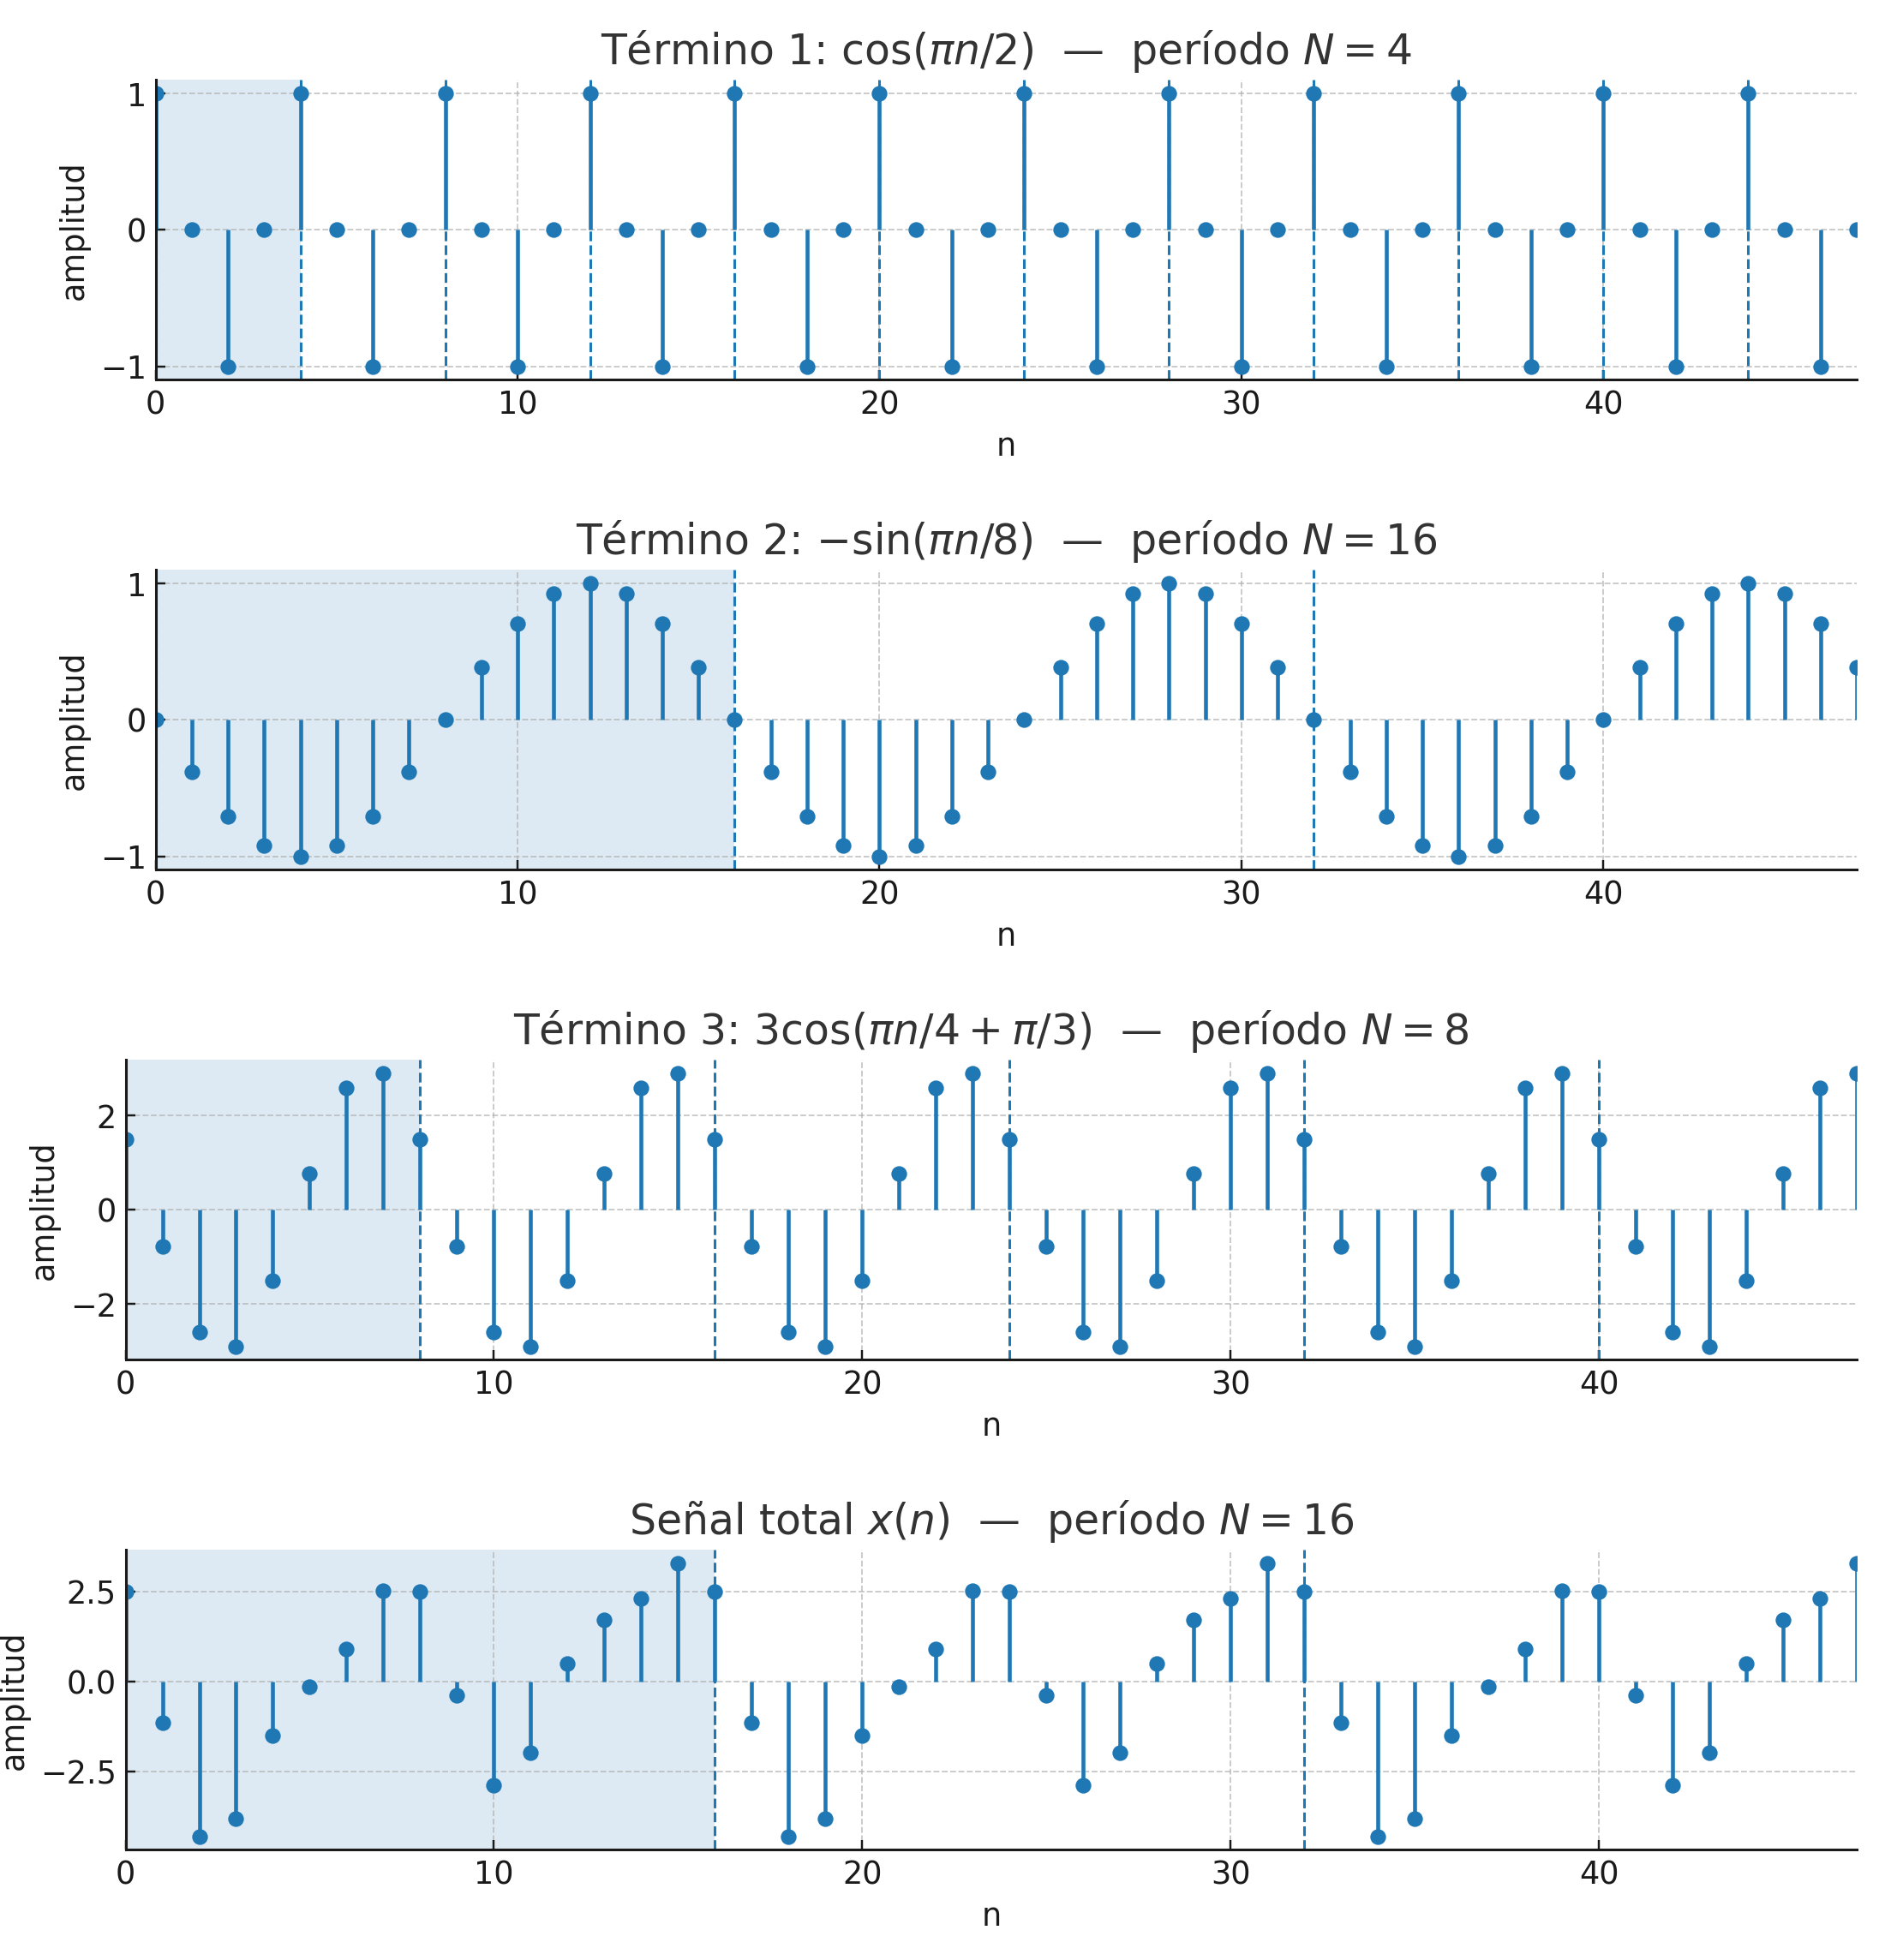
\includegraphics[width=0.4\textwidth]{Auxiliar_1_1}
    \caption{Esquema del corcho flotando (espacio reservado para la figura).}
    \label{fig:corcho}
\end{figure}

Para este ejercicio considere que existe una aceleración de gravedad $g$ y una fuerza de empuje dada por:
\begin{equation}
F_e = \rho g V
\end{equation}
donde $\rho$ es la densidad del agua y $V$ es el volumen del corcho sumergido.
    %%%%%%%%%%%%%%%%%%%%%%%%%%%
\begin{solution}

\subsection*{Resolución 1.1}

Definamos $y(t)$ como la posición del corcho medida desde el fondo del cilindro hacia arriba. El volumen sumergido del corcho será por lo tanto:
\begin{equation}
V = \pi R^2 (H - y)
\end{equation}

Ahora se deben identificar las fuerzas que actúan sobre el corcho son:
\begin{itemize}
    \item \textbf{La fuerza gravitacional}: $F_g = -mg$ (hacia abajo)
    \item \textbf{La fuerza de empuje}: $F_e = \rho g V = \rho g \pi R^2 (H - y)$ (hacia arriba)
\end{itemize}

Luego utilizando la segunda ley de Newton:
\begin{align}
m\ddot{y} &= -mg + \rho g \pi R^2 (H - y)
\end{align}

Recordemos que la condicion de equilibrio hace referencia a cuando un sistema está en reposo por lo que esto implica que $\ddot{y} = \dot{y} = 0$.
\begin{align}
0 &= -mg + \rho g \pi R^2 (H - y_{\mathrm{eq}})\\
y_{\mathrm{eq}} &= \frac{-mg}{\rho g \pi R^2} + H\\
y_{\mathrm{eq}} &= H - \frac{m}{\rho \pi R^2}
\end{align}
Con lo que se obtiene la posición de equilibrio del corcho.
\subsection*{Resolución 1.2}

Cuando el Corcho es perturbado, se debera utilizar la ecuacion del movimiento armónico simple (M.A.S.), la cual corresponde a lo siguiente:
\begin{equation}
m\ddot{y} = -mg + \rho g \pi R^2 (H - y)
\end{equation}
Reordenando la expresión se tiene:
\begin{equation}
\ddot{y} + \frac{\rho g \pi R^2}{m} \left( y - \left( H - \frac{m}{\rho \pi R^2} \right) \right) = 0
\end{equation}
Luego se busca el resolver esta ecuación, para esto haremos el siguiente cambio de variables convenientes.

\begin{align}
    x &:= y - y_{\mathrm{eq}} \\
\dot{x} &:= \dot{y} \\
\ddot{x} &:= \ddot{y}
\end{align}
Recordemos por otro lado que $H - \frac{m}{\rho \pi R^2} = y_{\mathrm{eq}}$, por lo tanto tendremos que:

\begin{align}
    \ddot{y} + \frac{\rho g \pi R^2}{m} \left( y - \left( H - \frac{m}{\rho \pi R^2} \right) \right) &= 0\\
    \ddot{y} + \frac{\rho g \pi R^2}{m} \left( y - y_{\mathrm{eq}}\right) &= 0\\
    \ddot{x} + \frac{\rho g \pi R^2}{m} x &= 0\\
    \ddot{x} + \omega^2 x &= 0
\end{align}
Donde definimos como $\omega^2 = \frac{\rho g \pi R^2}{m}$ como la frecuencia angular del sistema. Para este tipo de ecuacion diferencial se conocen las soluciones de movimiento armónico simple (M.A.S.), la cual es:
\begin{align}
    x(t) &= A \cos(\omega t) + B \sin(\omega t)\\
\end{align}
Luego realizando el cambio de variables:
\begin{align}
    y(t) &= x(t) + y_{\mathrm{eq}}\\
    y(t) &= A \cos(\omega t) + B \sin(\omega t) + H - \frac{m}{\rho \pi R^2}
\end{align}
Donde la velocidad del corcho sera la derivada de la posición, la cual correspondera a:
\begin{align}
    \dot{y}(t) &= -A \omega \sin(\omega t) + \frac{v_0}{\omega} \omega \cos(\omega t)\\
    \dot{y}(t) &= -A \omega \sin(\omega t) + v_0 \cos(\omega t)
\end{align}
Tenemos presente dos constantes las cuales son A y B, las cuales se pueden determinar a partir de las condiciones iniciales del sistema. Si consideramos que en el tiempo $t=0$ el corcho se encuentra en la posición $y(0) = x_0$ y con una velocidad $\dot{y}(0) = v_0$, tenemos que:
\begin{align}
    y(0) = x_{0} &=  A\cos(0)+B\sin(0) + H - \frac{m}{\rho \pi R^2}\\
    &= A + H - \frac{m}{\rho \pi R^2} 
\end{align}
Con lo que se obtiene que el  valor de A vendra dado por:
\begin{align}
    A= x_0 - H + \frac{m}{\rho \pi R^2}
\end{align}
Por otro lado para la velocidad tendremos de manera analoga que:
\begin{align}
    \dot{y}(0) = v_{0} &= -A \omega \sin(0) + B \omega \cos(0) \\
    &= B \omega
\end{align}
Por lo que obtenemos que el valor de B vendra dado por:
\begin{align}
    B = \frac{v_0}{\omega}
\end{align}
Finalmente tendremos que la posición del corcho en función del tiempo sera:
\begin{align}
    y(t) &= A \cos(\omega t) + B \sin(\omega t) + H - \frac{m}{\rho \pi R^2}\\
    &= \left( x_0 - H + \frac{m}{\rho \pi R^2} \right) \cos(\omega t) + \frac{v_0}{\omega} \sin(\omega t) + H - \frac{m}{\rho \pi R^2}
\end{align}
Con lo que se obtiene la posición del corcho en función del tiempo.
\end{solution}
    %%%%%%%%%%%%%%%%%%%%%%%%%%%
\question Un bloque de masa $M$ se desliza sin fricción entre dos resortes de constantes de resorte $k$ y $2k$. Ambos resortes tienen largo natural nulo. El sistema está obligado a moverse solo a lo largo del eje de los resortes. Inicialmente, el bloque está en su posición de equilibrio, con una velocidad $V$ hacia la derecha.

\begin{enumerate}
    \item Calcule la frecuencia angular y la amplitud de las oscilaciones.
    \item Escriba una expresión para la posición del bloque en función del tiempo $x(t)$.
    \item  Considere que cuando el resorte de la derecha está en su máxima elongación se corta. Determine cuánto tiempo tarda el bloque en chocar con la pared izquierda.
\end{enumerate}

\begin{figure}[h!]
    \centering
    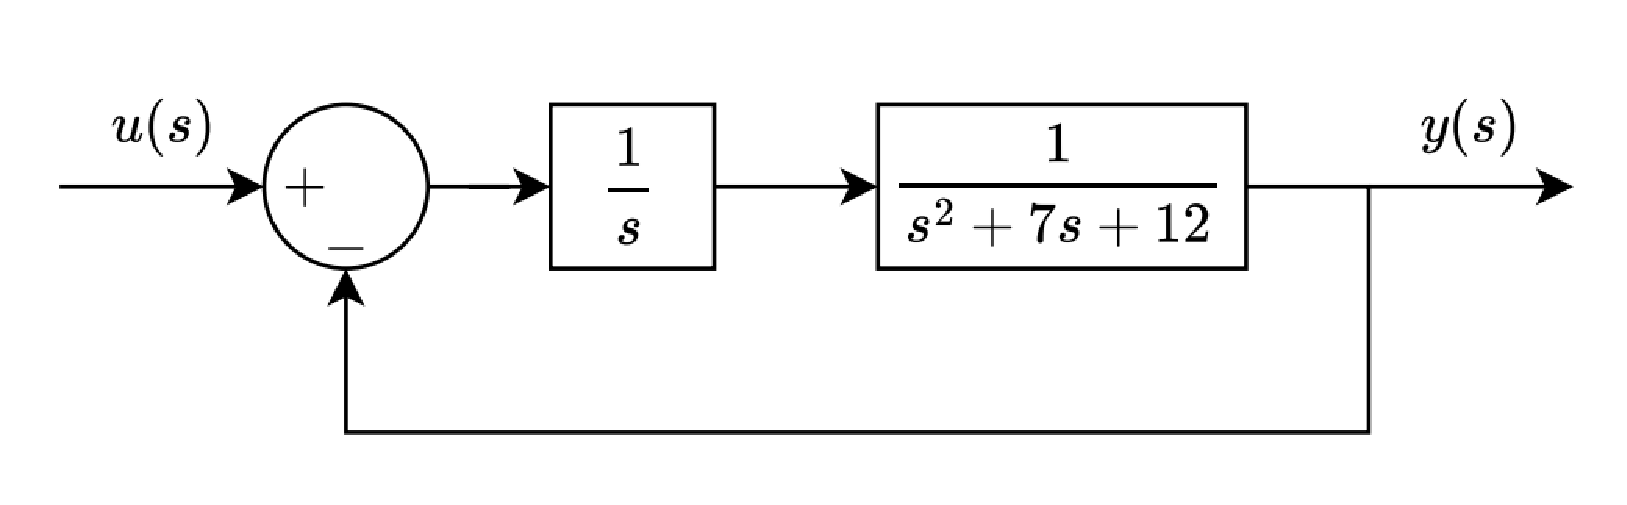
\includegraphics[width=.7\textwidth]{Auxiliar_1_2}
    \caption{Sistema masa–resortes (espacio reservado).}
    \label{fig:masa_resortes}
\end{figure}
%%%%%%%%%%%%%%%%%%%%%%%%%%
\begin{solution}

\subsection*{Resolución 2.1 }
Se busca calcular la frecuencia angular y la amplitud de las oscilaciones, para esto deberemos modelar el sistema mediante la segunda Ley de Newton. Por lo tanto tenemos que el diagrama de fuerzas vendra dado por:

\begin{center}
    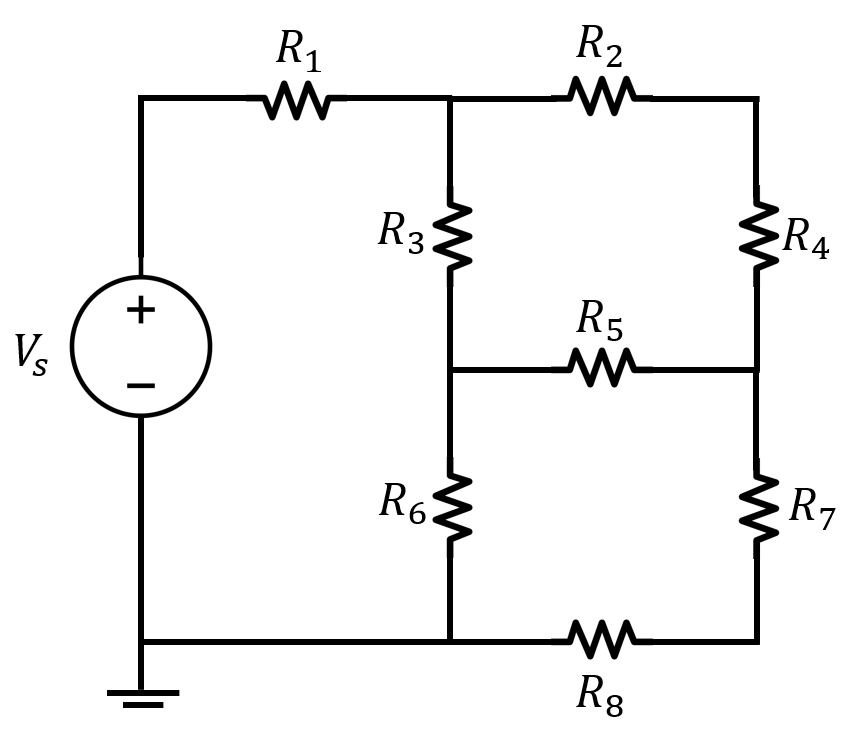
\includegraphics[width=.5\textwidth]{Auxiliar_1_3}
\end{center}
Luego tendremos que el sistema en equilibrio correspondera cuando $\ddot{x}=\dot{x}=0$. Por tanto:
\begin{align}
    \ddot{x}M &= F_{1} - F_{2}\\
    0 &= 2k(L-x)- kx\\
    0 &= -2kx + 2kL - kx\\
    0 &= -3kx + 2kL\\
    3kx &= 2kL\\
    x &= \frac{2L}{3}
\end{align}
Con lo que se obtiene el $x_{eq} = \frac{2L}{3}$. Luego considerando el sistema en general, tendremos que:
\begin{align}
    M\ddot{x} &= F_{1} - F_{2}\\
    M\ddot{x} &= 2k(L-x) - kx\\
    M\ddot{x} &= 2kL - 3kx
\end{align}
Luego tenemos que realizando el cambio de variable conveniente dado por:
\begin{align}
    y&:= x - x_{eq} = x - \frac{2L}{3}\\
    \dot{y} &:= \dot{x}\\
    \ddot{y} &:= \ddot{x}
\end{align}
Con lo que tenemos que el sistema vendra dado por:
\begin{align}
    M\ddot{y} &= 2kL - 3k\left(y + \frac{2L}{3}\right)\\
    M\ddot{y} &= 2kL - 3ky - 2kL\\
    M\ddot{y} &= -3ky \\
    \ddot{y} &= -\frac{3k}{M}y
\end{align}
De esta manera podemos identificar que el sistema presenta un movimiento armónico simple con una frecuencia angular dada por:
\begin{align}
    \omega &= \sqrt{\frac{3k}{M}}
\end{align}
Y una amplitud que dependerá de las condiciones iniciales del sistema. Luego tendra una solucion conocida dada por:
\begin{align}
    y(t) &= A \cos(\omega t + \phi)\\
    \dot{y} &= -A \omega \sin(\omega t + \phi)
\end{align}
Por lo que deberemos obtener la amplitud de la oscilación en función de las condiciones iniciales. Para esto, evaluamos las condiciones iniciales en $t=0$, dado que por enunciado tenemos que en $t=0$ se encuentra en su posición de equilibrio, luego se tendra que:
\begin{align}
  y(t=0) = x_{eq} - x_{eq} =  A\cos(0 + \phi) = 0  \rightarrow \phi= \frac{\pi}{2}\\
  \dot{y}(t=0) = -A\omega\sin(0+ \phi) = -A\omega\sin\left(\frac{\pi}{2}\right)= V \rightarrow A = - \frac{V}{\omega}
\end{align}
Con lo que finalmente obtenemos la expresion final dada por:
\begin{align}
    y(t) &= -\frac{V}{\omega} \cos\left(\omega t + \frac{\pi}{2}\right)\\
        &= \frac{V}{\omega} \sin(\omega t)
\end{align}
Donde la amplitud de oscilacion viene dada por
\begin{align}
    |A| = \frac{V}{\omega}
\end{align}
Devolviendonos sobre el cambio de variable tenemos que:
\begin{align}
    x(t) &= y(t) + X_{eq}\\
    &= \frac{V}{\omega} \sin(\omega t) + \frac{2L}{3}
\end{align}
\subsection*{Resolución 2.2}
Dado que el resorte de la derecha se corta, el la masa queda atada al resorte de constante elastica K desarrollando un MAS. Este mas es en torno a una nueva posicion de dequilibrio, la cual dado que tenemos un largo natural nulo sera $x_{eq} = 0$, con frecuencia angular $\omega = \frac{k}{m}$ y periodo 
\begin{align}
    T= \frac{1}{f} = \frac{2\pi}{\omega} = 2\pi \sqrt{\frac{M}{k}}
\end{align}
El periodo T se refiere a un ciclo completo, se demorara entonces 1/4 de ese tiempo en chocar la pared izquierda.

\end{solution}
%%%%%%%%%%%%%%%%%
\question Una cavidad óptica, elemento básico para construir un láser, puede hacerse usando un espejo plano y uno esférico cóncavo como se muestra en la siguiente figura.

\begin{figure}[h!]
    \centering
    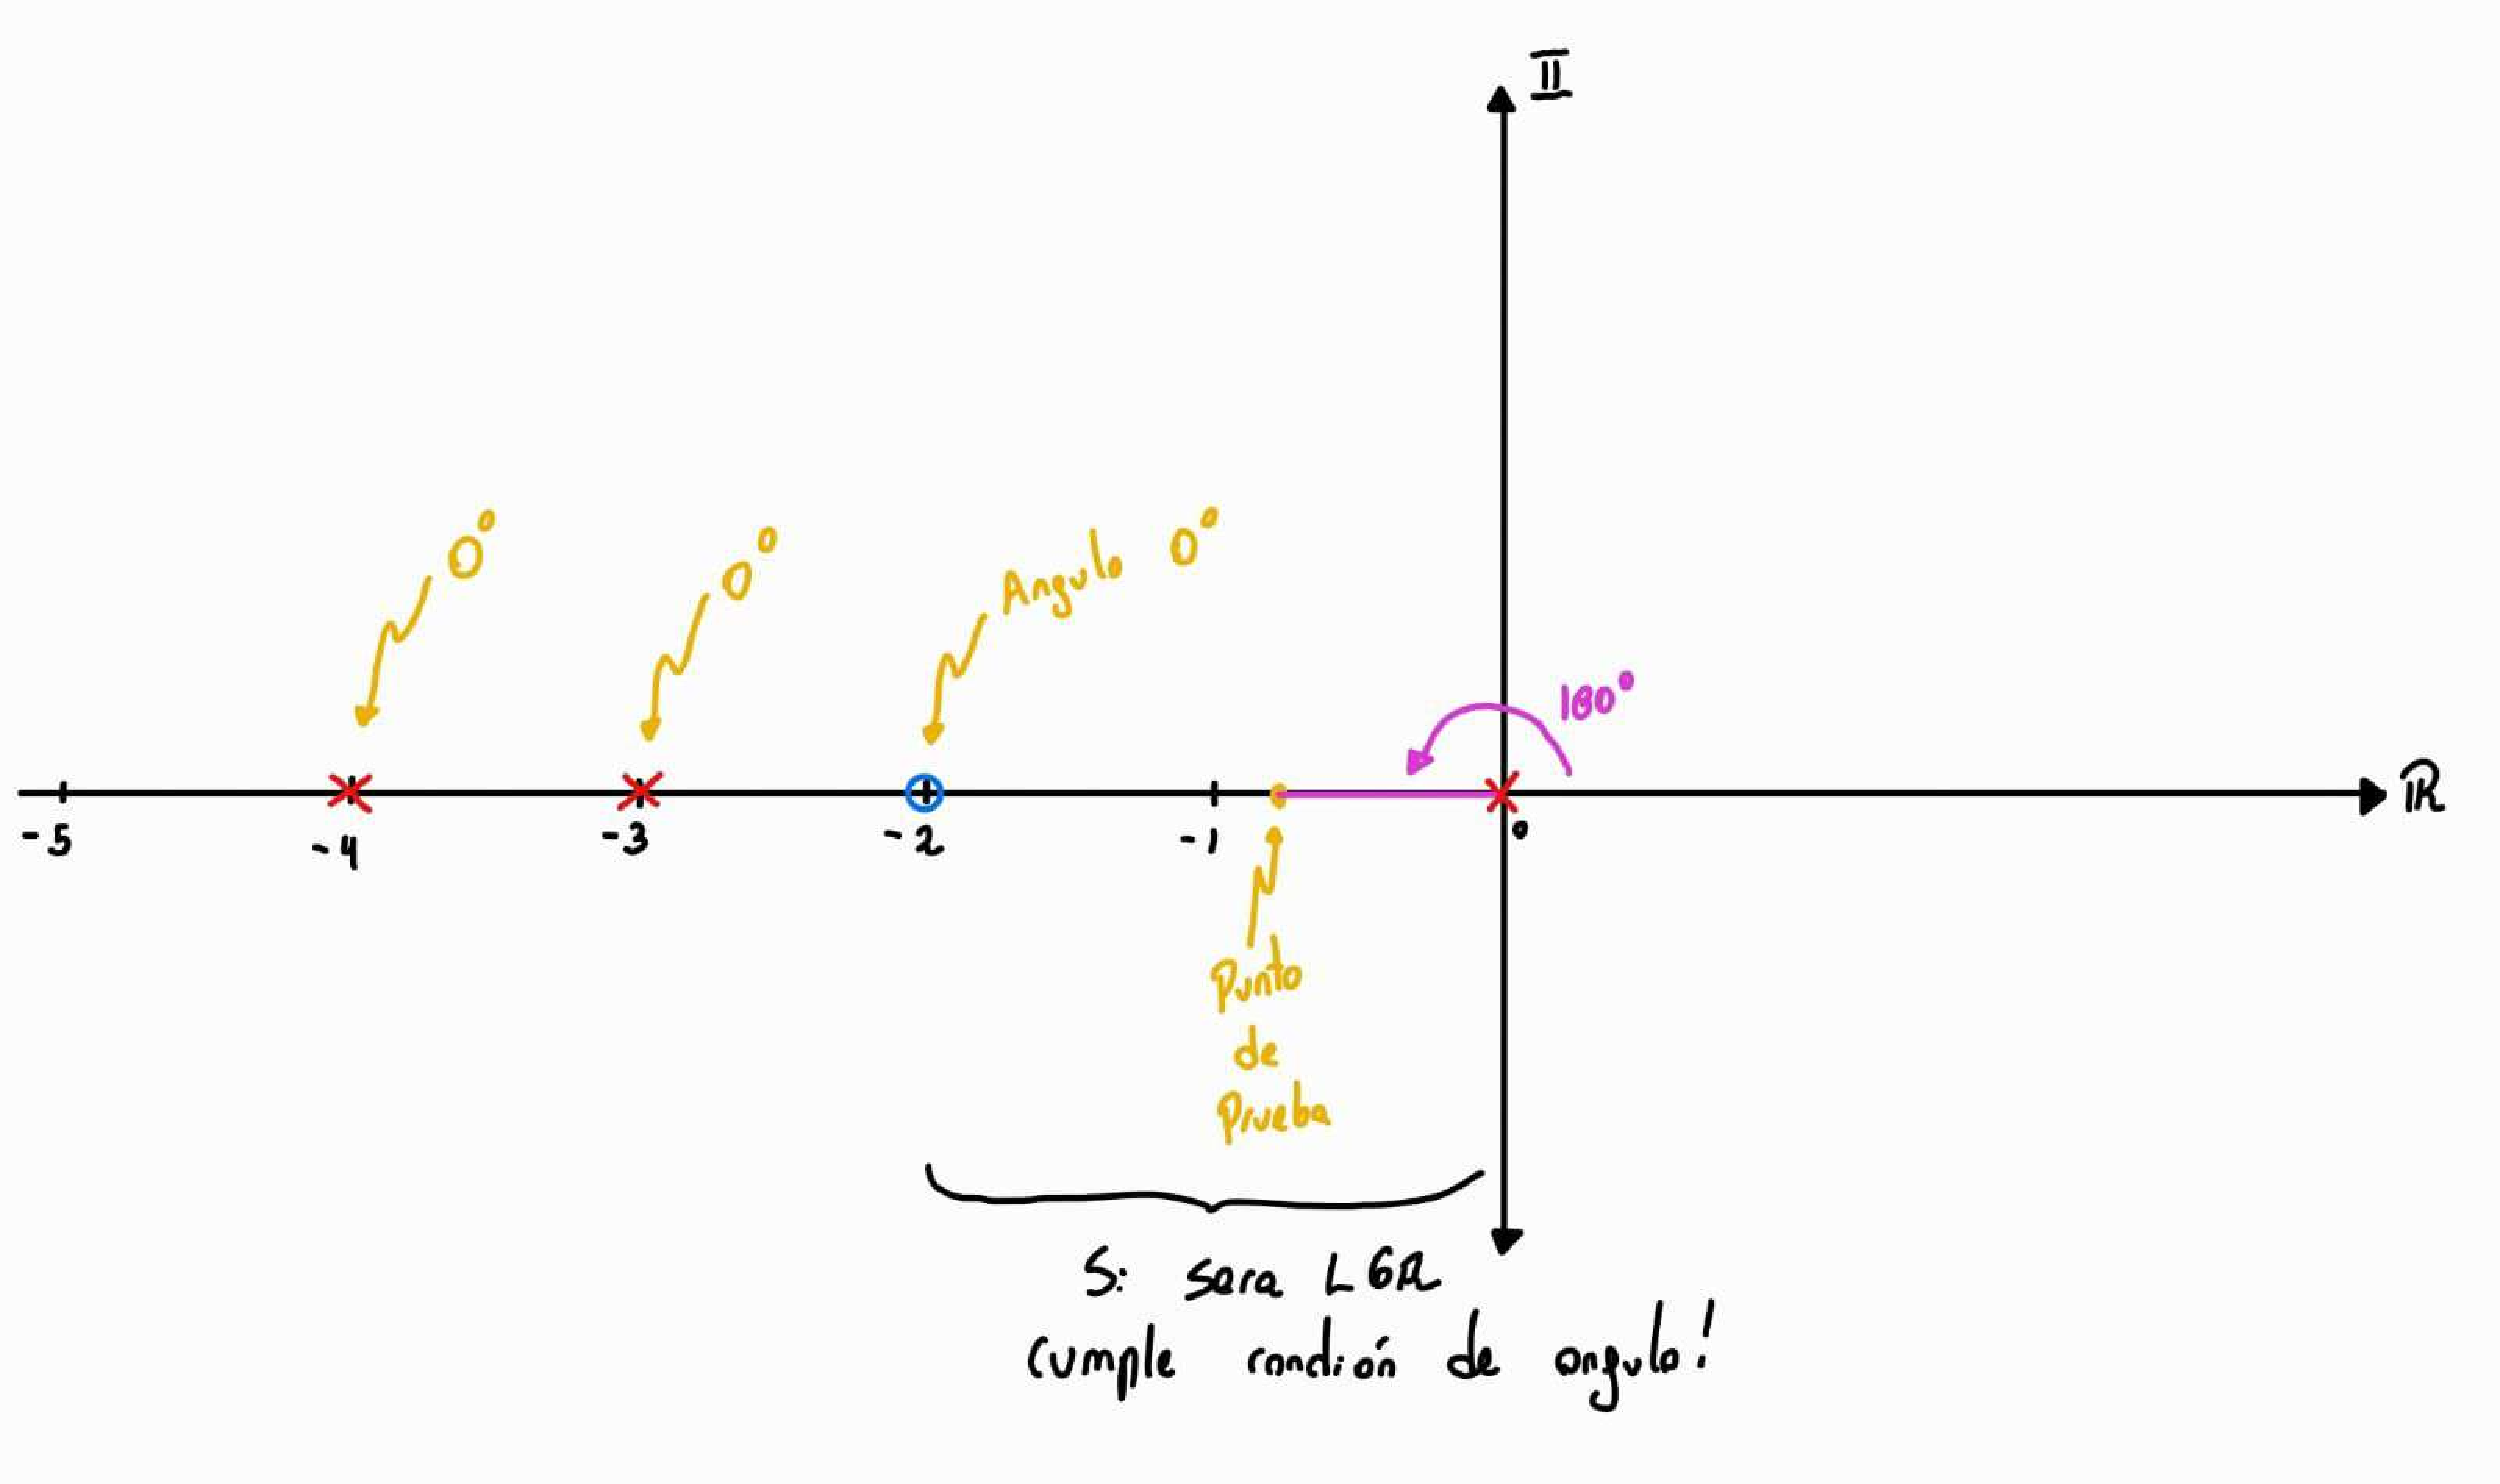
\includegraphics[width=0.6\textwidth]{Auxiliar_1_5}
    \caption{Un espejo plano frente a uno cóncavo.}
    \label{fig:cavidad_optica}
\end{figure}

\begin{enumerate}
    \item Si ponemos un peón de ajedrez entre los dos espejos tal que las distancias al espejo 1 (plano) y al espejo 2 (cóncavo) son $s_1=5\,[\mathrm{m}]$ y $s_2=20\,[\mathrm{m}]$, respectivamente, el radio de curvatura del cóncavo es $R=10\,[\mathrm{m}]$ y la altura del peón es $h_1=5\,[\mathrm{cm}]$, encuentre las imágenes del peón debidas a ambos espejos. ¿Son reales? ¿Están invertidas? ¿Cuál es su tamaño?
    \item Utilice estas dos imágenes como nuevos objetos para así generar dos nuevas imágenes. Si sigue haciendo esto muchas veces entenderá por qué se ven infinitas imágenes cuando se ponen dos espejos uno frente al otro.
\end{enumerate}

\begin{solution}
\subsection*{Resolución 3.1}
Recordemos que las ecuaciones que determinan a los espejos vienen dadas por:
\begin{align}
    \frac{1}{s}+\frac{1}{s'}=\frac{2}{R}=\frac{1}{f}
\end{align}
Donde debemos recordar la siguiente convención de signos:
\begin{center}
\begin{tabular}{c|c|c}
	\textbf{Magnitud} & $\boldsymbol{>0}$ & $\boldsymbol{<0}$ \\
\hline
$s$ (objeto) & objeto real & objeto virtual \\
$s'$ (imagen) & imagen real & imagen virtual \\
$R$ & espejo cóncavo & espejo convexo \\
$f$ & espejo cóncavo & espejo convexo \\
\end{tabular}
\end{center}
Donde tenemos que la magnificacion la cual se define como $m=-\frac{s'}{s}$ y se entiende como cuanto \textbf{crece} o \textbf{disminuye} la imagen respecto al objeto, esto puede relacionarde de manera directa con la altura como $h' = mh$.Luego para resolver el problema se tiene el siguiente esquema 
\begin{center}
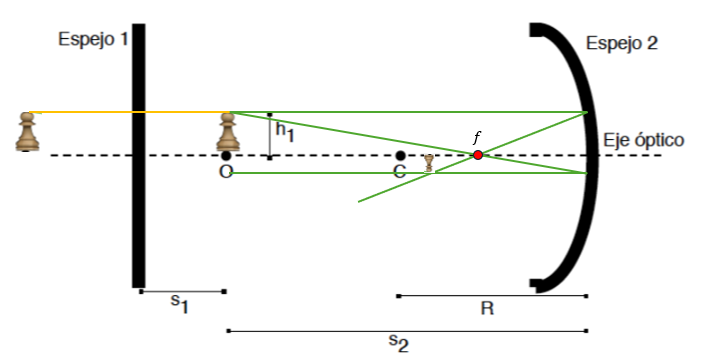
\includegraphics[width=0.8\textwidth]{Auxiliar_1_6}
\end{center}
\paragraph{Espejo 1 (plano).} Para un espejo plano $R\to\infty$ y por tanto
\[
\frac{1}{s_1}+\frac{1}{s_1'}=0\;\Rightarrow\; s_1'=-s_1=-5\,\text{m}.
\]
La imagen es \textbf{virtual} (detrás del espejo), \textbf{derecha} y del \textbf{mismo tamaño} porque
\[
m_1=-\frac{s_1'}{s_1}=1,\qquad h_1'=m_1h_1=h_1=5\,\text{cm}.
\]

\paragraph{Espejo 2 (cóncavo).} Dado $R=10\,\text{m}$, su foco es $f=R/2=5\,\text{m}$. Con $s_2=20\,\text{m}$:
\[
\frac{1}{s_2'}=\frac{1}{f}-\frac{1}{s_2}=\frac{1}{5}-\frac{1}{20}=\frac{3}{20}
\;\Rightarrow\; s_2'=\frac{20}{3}\,\text{m}\approx6.67\,\text{m}.
\]
Como $s_2'>0$, la imagen es \textbf{real} (frente al espejo cóncavo). El aumento es
\[
m_2=-\frac{s_2'}{s_2}=-\frac{\tfrac{20}{3}}{20}=-\frac{1}{3},
\]
por lo que la imagen está \textbf{invertida} y es \textbf{más pequeña}:
\[
h_2'=m_2h_1=-\tfrac{1}{3}\,\times 5\,\text{cm}=-\frac{5}{3}\,\text{cm}\approx-1.67\,\text{cm}.
\]

\subsection*{Resolución 3.2}
Si tratamos cada imagen obtenida (la virtual del espejo plano y la real del cóncavo) como \emph{nuevo objeto} para el espejo opuesto, cada una generará a su vez otra imagen; esas nuevas imágenes vuelven a actuar como objetos, y así sucesivamente. El proceso se repite indefinidamente y produce una \textbf{sucesión infinita de imágenes}, tal como se observa al enfrentar dos espejos.
\end{solution}
\end{questions}
\end{document}